\documentclass[onecolumn,aps, pre,amsmath,amssymb,longbibliography,12pt]{revtex4-2}
\usepackage{graphicx}
% \usepackage{dcolumn}
\usepackage{bm}
\usepackage{amsfonts}
\usepackage{xcolor,tabu}
\usepackage{multirow}
\usepackage{amsthm}
\usepackage{textcomp}
\usepackage{tikz}
\usepackage[colorlinks=true,
            linkcolor=blue,
            urlcolor=blue,
            citecolor=blue]{hyperref}
\hypersetup{bookmarksopen=true}
\usepackage{xr}
\usepackage{float}

\begin{document}
\title{Goals of the double emulsion study}
\maketitle

This note will be updated regularly to record my thoughts on the double emulsion project.
The goal of the study is not very clear, as all the research projects I have worked on in the past.
In particular, the topic to which I can make leading contribution has not become obvious.

The Chilean group of Profs. Soto and Cordero have done extensive experimental and theoretical work on the diffusion of inner drops.
During this postdoc, I will first follow up with their study.
I can contribute and gain an authorship, as well as familiarize me with the experimental system so I can develop other topics.

\section{Diffusion of inner drops}

An O/W/O double emulsion naturally forms a confined active bath with a passive object in it.
The dynamics of the inner drops is different from that in bulk due to the abnormal dynamics of bacteria under confinement.

My contribution in this topic will be to elucidate the dynamics of the inner drops.
The inner drops in our double emulsion system consist of 98\% hexadecane and 2\% SPAN80 surfactant.
Hexadecane is lighter than water, hence the inner drops always float to the top of the outer drops.
Pushed by swimming bacteria, the inner drops are fluctuating around the apex of the out drops.
The fluctuations are stronger than pure brownian motion.

Cristian is trying to compare his simulation with experiment.
A key issue in the way is the dynamics of the inner drops.
There dynamics can be classified into two different pathways: ``slide on the wall'' and ``detach from the wall''.
This is illustrated in Fig.~\ref{fig:pathways}.
In his simulations, the inner drop constantly detach from the surface of outer drops.
If we can confirm this behavior in experiment, it would provide an interesting aspect for comparison.
On the contrary, if we can confirm that the inner drops are always sliding on the wall, the model needs to be modified.
Either way, the progress of this project relies on the experimental investigation of the dynamics of the inner drops.

\begin{center}
  \begin{figure}
    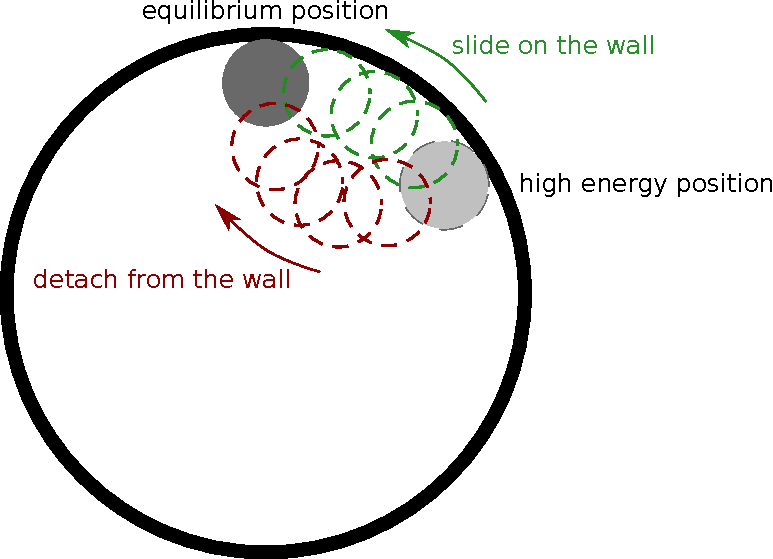
\includegraphics[width=3in]{pathways.pdf}
    \caption{Two possible dynamics of liquid drops in confined active bath.}
    \label{fig:pathways}
  \end{figure}
\end{center}

\end{document}
